%test.tex
\documentclass{article}
\usepackage{CJKutf8}
\usepackage{amsmath}
\usepackage{graphicx}
\usepackage{subfigure}
\usepackage[colorlinks,linkcolor=red]{hyperref}
\begin{CJK}{UTF8}{gbsn}
\title{非监督学习}
\author{布衣之莠}

\usepackage{listings}
\usepackage{color}

\definecolor{dkgreen}{rgb}{0,0.6,0}
\definecolor{gray}{rgb}{0.5,0.5,0.5}
\definecolor{mauve}{rgb}{0.58,0,0.82}

\lstset{frame=tb,
  language=Python,
  aboveskip=3mm,
  belowskip=3mm,
  showstringspaces=false,
  columns=flexible,
  basicstyle={\small\ttfamily},
  numbers=none,
  numberstyle=\tiny\color{gray},
  keywordstyle=\color{blue},
  commentstyle=\color{dkgreen},
  stringstyle=\color{mauve},
  breaklines=true,
  breakatwhitespace=true,
  tabsize=3
}
\begin{document}
\maketitle
\section{几种算法:}
\subsection{RBM:}
基于能量(Energy-based)的模型\\
Restricted Bolzmann Machines(RBM,1986,Hiton)\\
Deep Brief Network(DBN,2006,Hinton)
\subsection{AE:}
Auto-Encoder\\
Denoising AE\\
Stacked AE\\
Sparsing AE\\
Variational AE(VAE,生成样本)
\subsection{Cluster:}
K-means\\
Mean-shift\\
Spectral clustering(谱聚类)\\
Hieraechical clustering\\
Density-Based Spatial Clustering of Applications with Noise(DBSCAN)\\
Blanced Iterative Reducing and Clustering(Birch)\\
\subsection{Dimensionality reduction:}
Singular value decomposition(SVD)\\
Principal component analysis(PCA),KernelPCA,SparsePCA\\
Independent component analysis(ICA),Kernel ICA\\
Linear Discriminant Analysis(LDA)\\
Factor Analysis\\
Non-negative matrix factorization(NMF)\\
Stochastic neighbor embedding(SNE,2002,Hinton),对称SNE,t-SNE,LargeVis(唐建),注:用于低维空间可视化\\
Dictionary Learning(Sparse Representation)\\
Manifold Learning:\textit{MDS(Multidimensional Scaling),ISOMAP(Isometric feature mapping),LLE(Locally linear embedding),LE(Laplacian Eigenmap)}
\subsection{GAN:}
生成样本\\
DCGAN\\
WGAN\\
InfoGAN\\
\\

\section{受限波尔兹曼机}
\subsection{RBM}
RBM结构:
\begin{figure}[h]
\centering
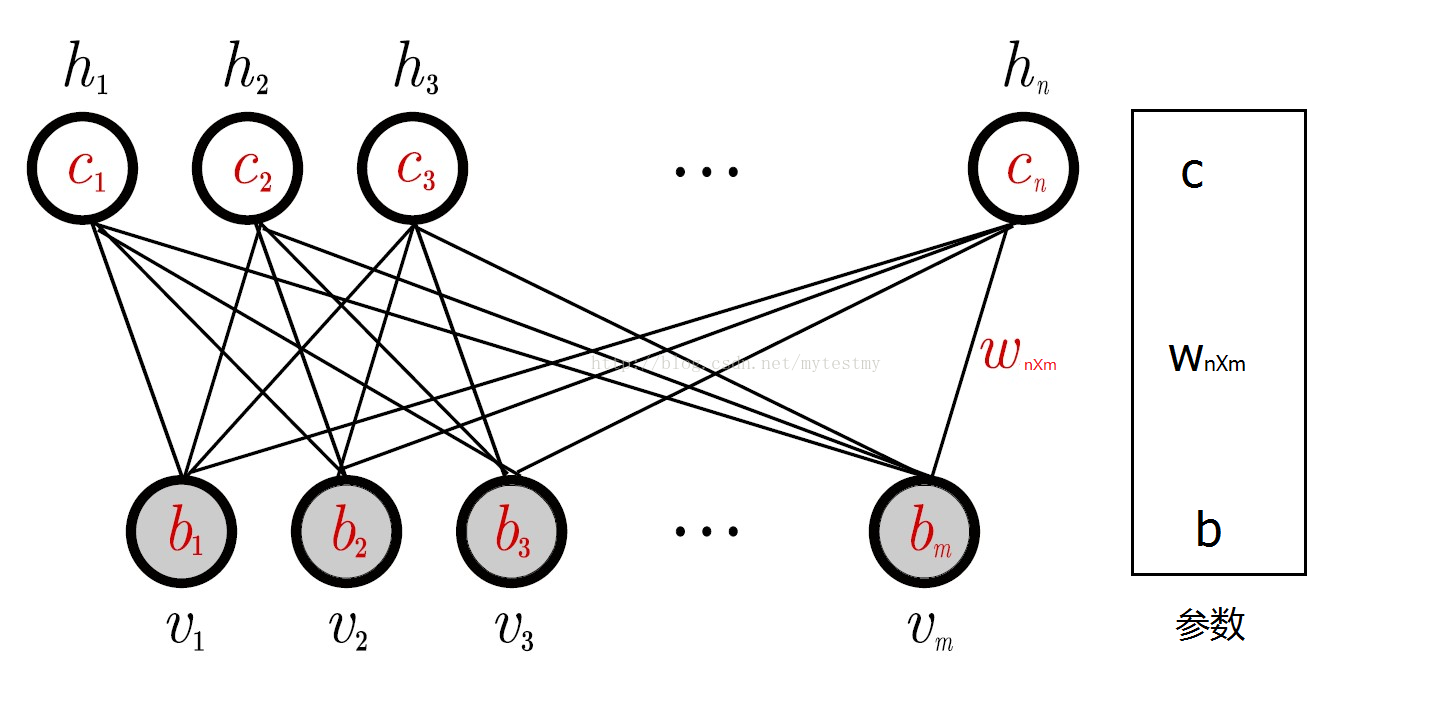
\includegraphics[width=0.8\linewidth]{1.png}
\caption{RBM}
\end{figure}\\

RBM网络结构有m个可视节点和n个隐藏节点,可视层和隐藏层之间的权重矩阵为$W_{m \times n}$,可视节点的bias为$b=(b_1,b_2,\dots,b_m)$,隐藏节点的bias为$c=(c_1,c_2,\dots,c_n)$。
RBM可以用于降维,用于初始化神经网络参数。\\
基于能量的模型。
能量函数定义如下:
\begin{equation}
E(v,h)=-\sum_{i=1}^{n}\sum_{j=1}^{m}w_{ij}h_iv_j-\sum_{j=1}^{m}b_jv_j-\sum_{i=1}^{n}c_ih_i \tag{2.1.1}
\end{equation}

定义可视节点和隐藏节点的联合概率为:
\begin{equation}
P(v,h)= \frac{e^{-E(v,h)}}{\sum_{v,h}e^{-E(v,h)}} \tag{2.1.2}
\end{equation}

这样定义的概率符合Gibbs分布。\\

条件概率和边缘概率是:
\begin{equation}
P(v)= \frac{\sum_he^{-E(v,h)}}{\sum_{v,h}e^{-E(v,h)}} \tag{2.1.3}
\end{equation}
\begin{equation}
P(h)= \frac{\sum_ve^{-E(v,h)}}{\sum_{v,h}e^{-E(v,h)}} \tag{2.1.4}
\end{equation}
\begin{equation}
P(v|h)=\frac{e^{-E(v,h)}}{\sum_he^{-E(v,h)}} \tag{2.1.5}
\end{equation}
\begin{equation}
P(h|v)=\frac{e^{-E(v,h)}}{\sum_ve^{-E(v,h)}} \tag{2.1.6}
\end{equation}

从概率到最大似然,最大似然定义:
\begin{equation}
L(\theta)=\frac{1}{N}\sum_{n=1}^N\ln P_{\theta}(v_n) \tag{2.1.7}
\end{equation}

可以通过梯度下降来最大化$L(\theta)$\\
对于每个$\ln p(v)$
\begin{equation}
\begin{aligned}
\frac{\partial \ln p(v)}{\partial W_{ij}} \\&=\sum_hp(h|v)h_iv_j-\sum_{v,h}p(v,h)h_iv_j \\&= \sum_hp(h|v)h_iv_j-\sum_vp(v)\sum_hp(h|v)h_iv_j \\&=p(h_i=1|v)v_j-\sum_vp(v)p(h_i=1|v)v_j
\end{aligned}
\tag{2.1.8}
\end{equation}
其中:
\begin{equation}
p(h_i=1|v)=\frac{\sum_{h_k \neq i}p(h_i,h_{k\neq i},v)}{\sum_hp(v,h)}=\sigma(\sum_{j=1}^mw_{ij}v_j+c_i) \tag{2.1.9}
\end{equation}

可以轻易求解,但第二项就要遍布所有$v$值,这样很麻烦。
\\

我们可以通过对训练样本抽样得到符合模型Gibbs分布的样本,然后直接用这些样本估算以上条件概率\\
对每个训练样本x,都用某种抽样方法抽取一个它对应的符合RBM网络表示的Gibbs分布的样本(对应的意思就是符合参数确定的Gibbs分布p(x)的),假如叫y;那么,对于整个的训练集${x_1,x_2,…x_n}$来说,就得到了一组符合RBM网络表示的Gibbs分布的样本${y_1,y_2,…,y_n}$,然后拿这组样本去估算第二项,那么梯度就可以用下面的公式来近似了:
\begin{equation}
\begin{aligned}
\frac{\partial \ln p(v)}{\partial W_{ij}}  \\&=p(h_i=1|v)v-\sum_vp(v)p(h_i=1|v)v \\& = p(h_i=1|v)v-\frac{1}{n}\sum_{j=1}^np(h_i=1|v_y)v_{yj}
\end{aligned}
\tag{2.1.10}
\end{equation}

我们有了上面的条件概率,我们就可以交替地进行下面的采样: \\
$h_0∼p(h|v_0),v_1∼p(v|h_0) \\
h_1∼p(h|v_1) v_2∼p(v|h_1) \\
\cdots  v_{k+1}∼p(v|h_k)$\\

在抽样步数k足够大的情况下,就可以获得符合RBM模型Gibbs分布的样本,得到这些样本就可以计算梯度的第二项了。

通过Constrastive Divergence来学习\\
\begin{figure}[h]
\centering
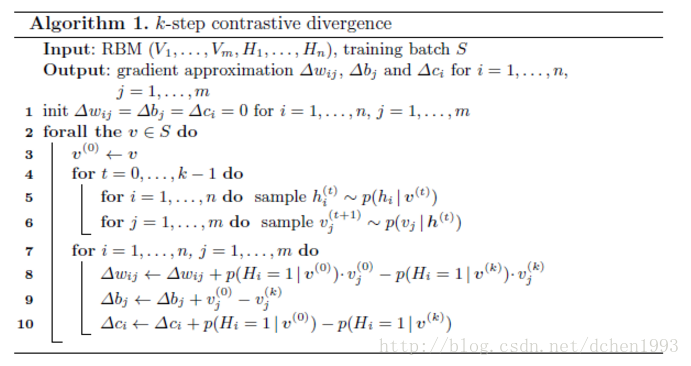
\includegraphics[width=0.8\linewidth]{3.png}
\caption{CD-K算法}
\end{figure}\\
参考:\\
\href{http://lib.csdn.net/article/deeplearning/59097?knId=1746}{限制波尔兹曼机}\\
\href{http://deeplearning.net/tutorial/rbm.html#rbm}{深度学习教程theano实现限制波尔兹曼机}
\subsection{DBN}
Deep Brief Network

把原始数据输入到最下面的RBM可视层中,然后训练RBM1,训练完成之后把RBM1的隐含层作为RBM2的可视层,继续训练RBM2,接下来把RBM2的隐含层做为RBM3的可视层,直到训练完成为止。RBM的最后一隐含层层与输出层连接,对该层进行bp优化。
\begin{figure}[h]
\centering
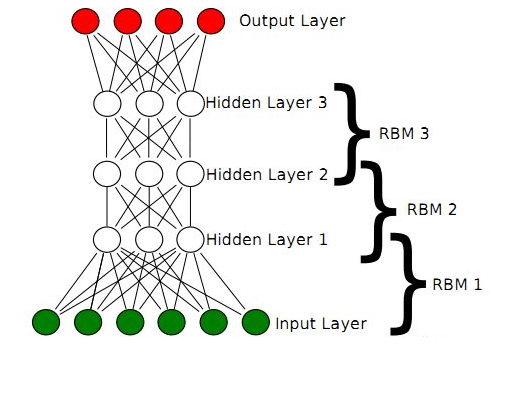
\includegraphics[height=0.5\linewidth]{2.png}
\caption{DBN}
\end{figure}
参考:\href{}{深度信念网络}



\section{自编码器}
\subsection{AutoEncoder}
AE结构
\begin{figure}[h]
\centering
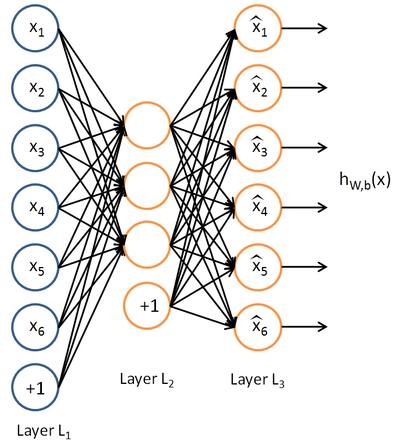
\includegraphics[height=0.5\linewidth]{4.png}
\caption{AutoEncoder}
\end{figure}\\
自编码神经网络尝试学习一个 $\textstyle h_{W,b}(x) \approx x$ 的函数。它尝试逼近一个恒等函数,从而使得输出 $\textstyle \hat{x}$ 接近于输入 $\textstyle x$ 。当我们为自编码神经网络加入某些限制,比如限定隐藏神经元的数量,自编码神经网络可以去学习输入数据的压缩表示。
\subsection{Denoising AE}
DAE(Denoising Autoencoder)的核心思想是,一个能够从中恢复出原始信号的神经网络表达未必是最好的,能够对“损坏”的原始数据编码、解码,然后还能恢复真正的原始数据,这样的特征才是好的。
\begin{figure}[h]
\centering
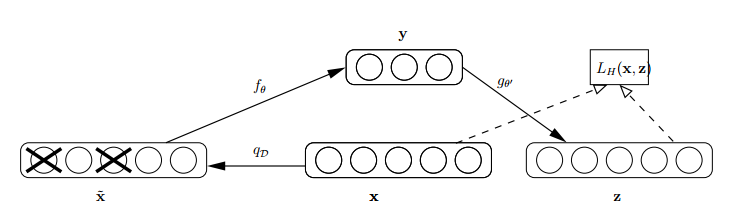
\includegraphics[width=0.8\linewidth]{5.png}
\caption{Denosing AE}
\end{figure}\\
参考:\\
\href{https://www.researchgate.net/publication/221346269_Extracting_and_composing_robust_features_with_denoising_autoencoders}{Extracting and Composing Robust Features with
Denoising Autoencoders}
\subsection{Stacked AE }
SAE:AE逐层堆叠, layer-wise unsuperwised pre-training 
\begin{figure}[h]
\centering
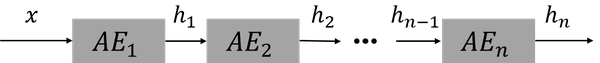
\includegraphics[width=0.8\linewidth]{6.png}
\caption{Stacked AE}
\end{figure}\\
多个稀疏自编码器与softmax分类器结合,构建一个包含多隐藏层与一个最终softmax分类器的SAE网络,其训练步骤如下\\
Step1:将原始数据作为 SAE 的输入,训练第一个隐藏层的网络参数,并用训练好的参数算出第一个隐藏层的输出;\\
Step2:把上一层网络的输出作为其下一层网络的输入,用同样的方法训练该层网络的参数;重复这一步骤,直到训练完最后一个隐藏层;\\
Step3:将 Step2 中的输出作为 softmax 分类器的输入,结合原始数据的标签来训练 softmax 分类器的网络参数;\\
Step4:计算整个网络(包括所有隐藏层和一个 softmax 分类器)的代价函数,以及该网络对每个参数的偏导函数值;\\
Step5:用 Step1,Step2 和 Step3 的网络参数作为整个深度网络的初始化参数值,然后用优化算法迭代求出代价函数最小值附近的参数值,并作为整个网络最后的最优参数值。\\
\subsection{Sparse AE}
AE隐藏神经元的数量较大,我们仍然通过给自编码神经网络施加一些其他的限制条件来发现输入数据中的结构。\\
\begin{figure}[h]
\centering
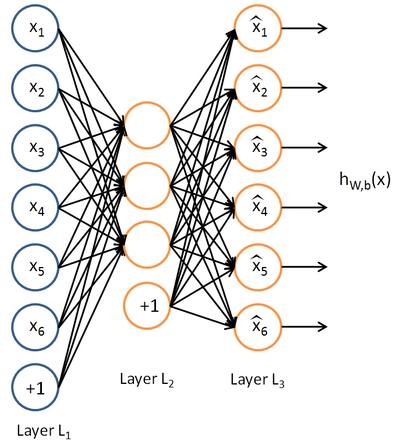
\includegraphics[height=0.5\linewidth]{4.png}
\caption{AutoEncoder}
\end{figure}\\
稀疏性限制:\\
神经元的输出接近于1的时候被激活,而输出接近于0的时候被抑制,那么使得神经元大部分的时间都是被抑制的限制则被称作稀疏性限制。假设的神经元的激活函数是sigmoid函数。tanh作为激活函数的话,当神经元输出为-1的时候,神经元是被抑制的。\\
我们将使用 $\textstyle a^{(2)}_j(x)$ 来表示在给定输入为 $\textstyle x $情况下,自编码神经网络隐藏神经元$ \textstyle j $的激活度。 进一步,让
$\hat\rho_j = \frac{1}{m} \sum_{i=1}^m \left[ a^{(2)}_j(x^{(i)}) \right]$
表示隐藏神经元 $\textstyle j $的平均活跃度(在训练集上取平均)。我们可以近似的加入一条限制
$\hat\rho_j = \rho,$
其中,$ \textstyle \rho$是稀疏性参数,通常是一个接近于0的较小的值(比如 $\textstyle \rho = 0.05$ )。

为了实现这一限制,我们将会在我们的优化目标函数中加入一个额外的惩罚因子,而这一惩罚因子将惩罚那些 $\textstyle \hat\rho_j $和 $\textstyle \rho $有显著不同的情况从而使得隐藏神经元的平均活跃度保持在较小范围内。惩罚因子
$
\sum_{j=1}^{s_2} \rho \log \frac{\rho}{\hat\rho_j} + (1-\rho) \log \frac{1-\rho}{1-\hat\rho_j}.
$
这里, $\textstyle s_2 $是隐藏层中隐藏神经元的数量,而索引 $\textstyle j$ 依次代表隐藏层中的每一个神经元。
\\
参考:\\
\href{http://deeplearning.stanford.edu/wiki/index.php/Autoencoders_and_Sparsity}{UFLDL Tutorial}
\subsection{Variational AE}
变分自编码器
贝叶斯神经网络和变分推断
\begin{figure}[h]
\centering
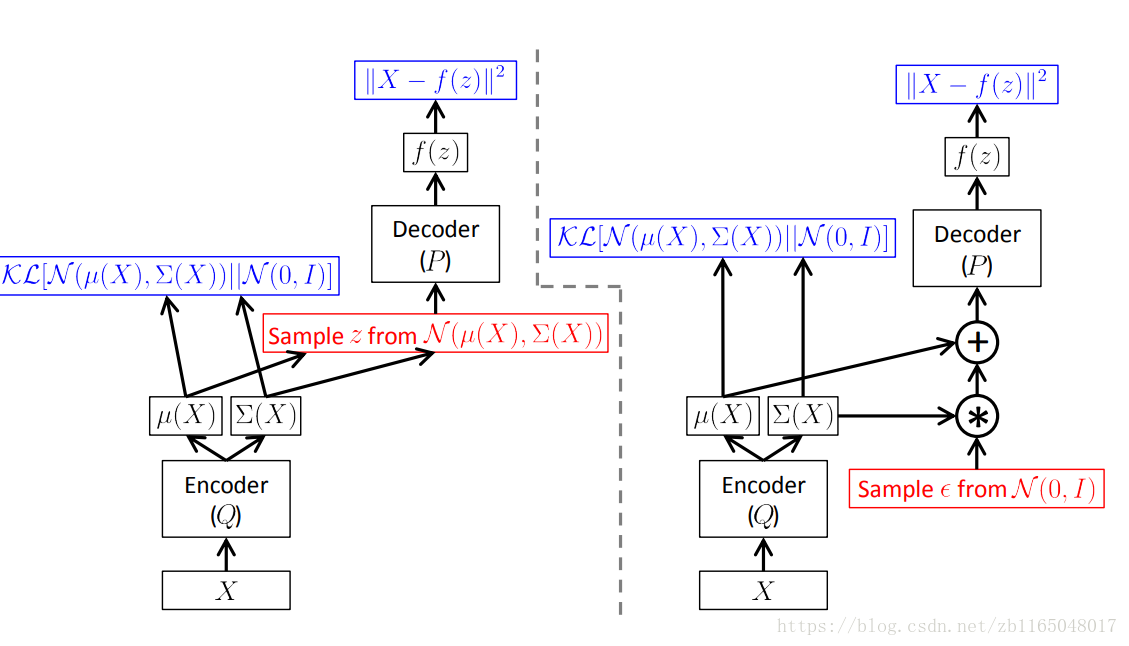
\includegraphics[height=0.5\linewidth]{7.png}
\caption{Variational AE}
\end{figure}\\
优化目标ELBO(Evidence Lower Bound)
\begin{equation}
ELBO=\log p(x)-KL[q(z|x)\parallel p(z|x)] \tag{3.5.1}
\end{equation}
可以简化为:
\begin{equation}
ELBO=E_{z \sim q}[\log p(x|z)] -KL(q(z|x) \parallel p(z))
\end{equation}
最终损失为:
\begin{equation}
L=\parallel X-f(z) \parallel ^2-\lambda*KL(q(z|x) \parallel p(z))
\end{equation}
重新参数化(reparameterization trick)\\
\begin{lstlisting}
class VAE(nn.Module):
    def __init__(self):
        super(VAE, self).__init__()

        self.fc1 = nn.Linear(784, 400)
        self.fc21 = nn.Linear(400, 20)
        self.fc22 = nn.Linear(400, 20)
        self.fc3 = nn.Linear(20, 400)
        self.fc4 = nn.Linear(400, 784)
        self.relu = nn.ReLU()
        self.sigmoid = nn.Sigmoid()

    def encode(self, x):
        h1 = self.relu(self.fc1(x))    
        return self.fc21(h1), self.fc22(h1)

    def reparametrize(self, mu, logvar):
        std = logvar.mul(0.5).exp_()#exp(0.5*var)
        eps = Variable(std.data.new(std.size()).normal_())
        return eps.mul(std).add_(mu)#eps*std+u

    def decode(self, z):
        h3 = self.relu(self.fc3(z))      
        return self.sigmoid(self.fc4(h3))

    def forward(self, x):
        mu, logvar = self.encode(x.view(-1, 784))#[ size 32x20 (GPU 0)],[size 32x20 (GPU 0)]
        z = self.reparametrize(mu, logvar)      
        return self.decode(z), mu, logvar

reconstruction_function = nn.BCELoss()
def loss_function(recon_x, x, mu, logvar):
    BCE = reconstruction_function(recon_x, x.view(-1, 784))
    # see Appendix B from VAE paper:
    # Kingma and Welling. Auto-Encoding Variational Bayes. ICLR, 2014
    # https://arxiv.org/abs/1312.6114
    # 0.5 * sum(1 + log(sigma^2) - mu^2 - sigma^2)
    KLD_element = mu.pow(2).add_(logvar.exp()).mul_(-1).add_(1).add_(logvar)
    KLD = torch.sum(KLD_element).mul_(-0.5)

    return BCE + KLD

\end{lstlisting}
参考:\\
\href{https://arxiv.org/pdf/1312.6114.pdf}{Auto-Encoding Variational Bayes}\\
\href{https://arxiv.org/pdf/1606.05908.pdf}{Tutorial on Variational Autoencoders} \\
\href{https://blog.csdn.net/zb1165048017/article/details/81773660}{变分自编码器}
\section{聚类}
Cluster,这一类了解的比较多,先搁置
\section{降维}
Dimensionality reduction
SVD,PCA,ICA,LDA,NMF先搁置
\subsection{字典学习}
稀疏表示:\\
假设我们用一个M*N的矩阵表示数据集X,每一行代表一个样本,每一列代表样本的一个属性,一般而言,该矩阵是稠密的,即大多数元素不为0。稀疏表示的含义是,寻找一个系数矩阵W(K*N)以及一个字典矩阵D(M*K),使得D*W尽可能的还原X,且W尽可能的稀疏。W便是X的稀疏表示。
周志华老师写的《机器学习》这本书上原文:“为普通稠密表达的样本找到合适的字典,将样本转化为合适的稀疏表达形式,从而使学习任务得以简化,模型复杂度得以降低,通常称为‘字典学习’(dictionary learning),亦称‘稀疏编码’(sparse coding)”
\begin{figure}[h]
\centering
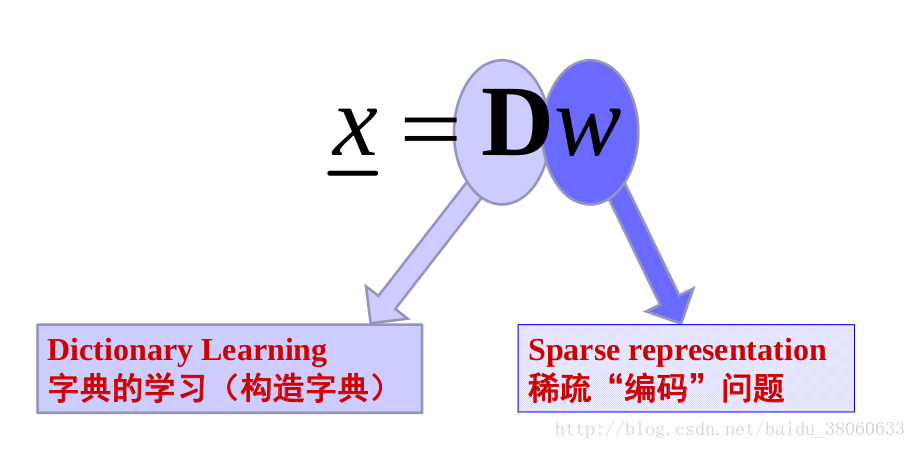
\includegraphics[height=0.4\linewidth]{9.png}
\caption{字典学习}
\end{figure}\\
表达为优化问题为
\begin{equation}
\min_{D,W} \sum_i \parallel x_i-DW_I \parallel_2^2+\lambda \sum_i \parallel W_i \parallel_1  \tag{5.1.1}
\end{equation}
上式中第一个累加项说明了字典学习的第一个目标是字典矩阵与稀疏表示的线性组合尽可能的还原样本;第二个累加项说明了alphai应该尽可能的稀疏。之所以用L1范式是因为L1范式正则化更容易获得稀疏解。原因可参考\href{https://blog.csdn.net/zouxy09/article/details/24971995/}{机器学习中的正则化}\\
该算法包含两个阶段:字典构建阶段(Dictionary Generate)和利用字典表示样本阶段(Sparse coding with a precomputed dictionary)。求解字典学习最优化问题的步骤为:\\
1.初始化字典D优化稀疏采样W。\\ 
2.在优化后的W上更新字典D。\\ 
重复上述两步,求得最终D以及X的稀疏表示W。\\
\begin{figure}[h]
\centering
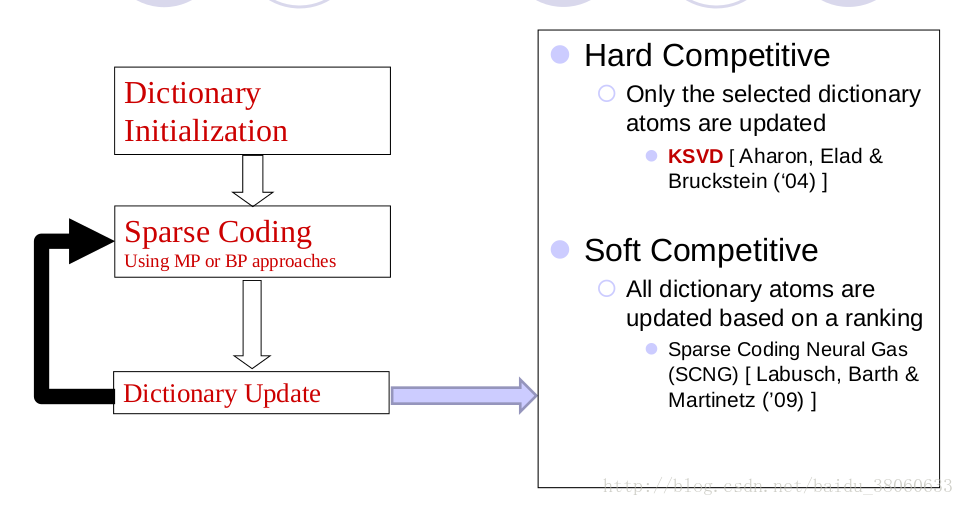
\includegraphics[height=0.4\linewidth]{10.png}
\caption{更新算法}
\end{figure}\\
参考:\\
\href{https://blog.csdn.net/baidu_38060633/article/details/70338345}{稀疏表示与字典学习}\\
\href{https://blog.csdn.net/hjimce/article/details/50810129}{字典学习与k-svd算法}\\
\href{https://scikit-learn.org/stable/modules/decomposition.html#dictionary-learning}{sklearn字典学习}
\subsection{流形学习}
非线性降维,可以参考周志华的机器学习中算法的详细步骤,此处给出基本思想。\\
流形:局部区域与欧式空间同胚的拓扑空间(连续的变换最后都能变成一样的两个物体,称为同胚,Homeomorphism)。
流形上的点本身是没有坐标的,所以为了表示这些数据点,我们把流形放入到外围空间(ambient space),用外围空间上的坐标来表示流形上的点,例如三维空间 $R^3$ 中球面是一个2维曲面,即球面上只有两个自由度,但我们一般采用外围空间$R^3$ 空间中的坐标来表示这个球面。
流行学习可以概括为:在保持流形上点的某些几何性质特征的情况下,找出一组对应的内蕴坐标(intrinsic coordinate),将流形尽量好的展开在低维平面上,这种低维表示也叫内蕴特征(intrinsic feature),外围空间的维数叫观察维数,其表示叫自然坐标,在统计上称为observation。流形学习假设所处理的数据点分布在嵌入于外维欧式空间的一个潜在的流形体上,或者说这些数据点可以构成这样一个潜在的流形体。假设数据是均匀采样于一个高维欧氏空间中的低维流形,流形学习就是从高维采样数据中恢复低维流形结构,即找到高维空间中的低维流形,并求出相应的嵌入映射,以实现维数约简或者数据可视化。\\
\textbf{ MDS(Multidimensional Scaling)多维尺度变换}\\
MDS的基本思想:约简后低维空间中任意两点间的距离应该与它们在原高维空间中的距离相同\\
参考:\\
\href{http://www.cnblogs.com/tanjuntao/p/8067748.html}{MDS实现}\\
\textbf{ISOMAP(Isometric feature mapping)等度量映射}\\
MDS算法的变种,其思想和MDS一样,只不过在计算高维空间的距离时是采用测地距离的,而不是无法真实的表达两点之间的欧式距离\\
\begin{figure}[h]
\centering
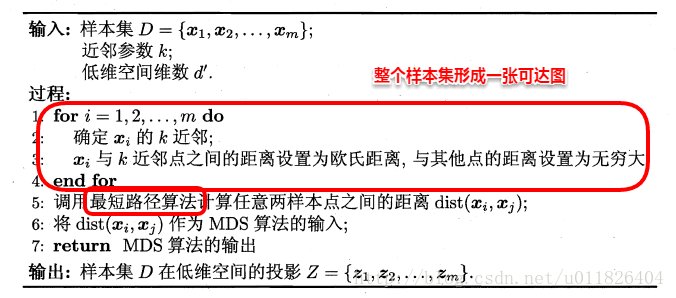
\includegraphics[height=0.4\linewidth]{11.png}
\caption{ISOMAP算法}
\end{figure}\\
\textbf{LLE(Locally Linear Embedding) 局部线性嵌入}\\
局部线性嵌入的思想:只是试图去保持领域内样本之间的关系。具体如下图所示,样本从高维空间映射到低维空间后,各个领域内的样本之间的线性关系不变。
\begin{figure}[h]
\centering
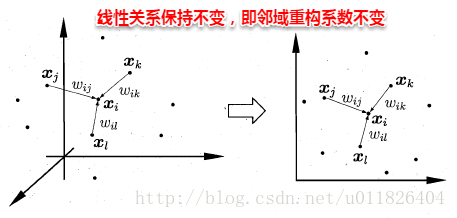
\includegraphics[height=0.4\linewidth]{13.png}
\caption{LLE算法}
\end{figure}\\
即样本点$x_i$的坐标能通过它的领域样本$x_j$,$x_l$,$x_k$重构出来,$x_i=w_{ij}x_j+w_{il}x_l+w_{ik}x_k$而这里的权值参数在低维和高维空间是一致的。\\
\textbf{LE (Laplacian Eigenmaps) 拉普拉斯特征映射}\\
基本思想:在高维空间中离的很近的点投影到低维空间中也应该离得很近。LE方法在黎曼几何的框架内,用邻接图来描述一个流形,并在映射到低维空间的过程中,保持了图的局部邻接关系。LE的基本思想就是用一个无向有权图来描述一个流形,然后通过用图的嵌入(graph embedding)来找低维表示。简单来说,就是保持图的局部邻接关系的情况把这个图从高维空间中重新画在一个低维空间中(graph drawing)。
\subsection{T-SNE}
看看这篇吧!\href{http://bindog.github.io/blog/2016/06/04/from-sne-to-tsne-to-largevis/}{从SNE到t-SNE再到LargeVis}
\section{对抗生成网络}
GAN
\end{CJK}
\end{document}